\documentclass[a4paper, 12pt]{report}
\usepackage{cmap}
\usepackage{amssymb}
\usepackage{amsmath}
\usepackage{graphicx}
\usepackage{amsthm}
\usepackage{upgreek}
\usepackage{setspace}
\usepackage{color}
\usepackage{moreverb}
\usepackage[T2A]{fontenc}
\usepackage[utf8]{inputenc}
\usepackage[normalem]{ulem}
\usepackage{mathtext} % русские буквы в формулах
\usepackage[left=2cm,right=2cm, top=2cm,bottom=2cm,bindingoffset=0cm]{geometry}
\usepackage[english,russian]{babel}
\usepackage[unicode]{hyperref}
\newenvironment{Proof} % имя окружения
{\par\noindent{$\blacklozenge$}} % команды для \begin
{\hfill$\scriptstyle\boxtimes$}
\newcommand{\Rm}{\mathbb{R}}
\newcommand{\Cm}{\mathbb{C}}
\newcommand{\Z}{\mathbb{Z}}
\newcommand{\I}{\mathbb{I}}
\newcommand{\N}{\mathbb{N}}
\newcommand{\rank}{\operatorname{rank}}
\newcommand{\Ra}{\Rightarrow}
\newcommand{\ra}{\rightarrow}
\newcommand{\FI}{\Phi}
\newcommand{\Sp}{\text{Sp}}
\renewcommand{\leq}{\leqslant}
\renewcommand{\geq}{\geqslant}
\renewcommand{\alpha}{\upalpha}
\renewcommand{\beta}{\upbeta}
\renewcommand{\gamma}{\upgamma}
\renewcommand{\delta}{\updelta}
\renewcommand{\varphi}{\upvarphi}
\renewcommand{\phi}{\upvarphi}
\renewcommand{\tau}{\uptau}
\renewcommand{\lambda}{\uplambda}
\renewcommand{\psi}{\uppsi}
\renewcommand{\mu}{\upmu}
\renewcommand{\omega}{\upomega}
\renewcommand{\d}{\partial}
\renewcommand{\xi}{\upxi}
\renewcommand{\epsilon}{\upvarepsilon}
\newcommand{\intx}{\int\limits_{x_0}^x}
\newcommand\Norm[1]{\left\| #1 \right\|}
\newcommand{\sumk}{\sum\limits_{k=0}^\infty}
\newcommand{\sumi}{\sum\limits_{i=0}^\infty}
\newtheorem*{theorem}{Теорема}
\newtheorem*{cor}{Следствие}
\newtheorem*{lem}{Лемма}
\begin{document}
	% Оформление титульного листа
	\begin{titlepage}
		\begin{center}
			\textsc{МИНИСТЕРСТВО ОБРАЗОВАНИЯ РЕСПУБЛИКИ БЕЛАРУСЬ БЕЛОРУССКИЙ ГОСУДАРСТВЕННЫЙ УНИВЕРСИТЕТ
				\\[5mm]
				ФАКУЛЬТЕТ ПРИКЛАДНОЙ МАТЕМАТИКИ И ИНФОРМАТИКИ\\[2mm]
				Кафедра информационных систем управления
			}
			
			\vfill
			
			\textbf{Отчет по лабораторной работе №2\\
				Вариант 22
				\\[26mm]
			}
		\end{center}
		
		\hfill
		\begin{minipage}{.5\textwidth}
			\begin{flushright}
				Бовта Тимофея Анатольевича\\
				студента 3 курса\\
				специальности «прикладная математика»\\[5mm]
				
				Преподаватель:\\[2mm] 
				Д. Ю. Кваша\\
			\end{flushright}
		\end{minipage}%
		\vfill
		\begin{center}
			Минск, 2024\ г.
		\end{center}
	\end{titlepage}
	\newpage
	\section*{Лабораторная работа №2}
	\subsection*{Описание задачи.}
	Строительный магазин столкнулся со следующей проблемой. Клиентам нужен оргалит размером 120 × 90 см$^2$, 120 × 150 см$^2$ и 120 × 180 см$^2$ в количестве не менее 20, 50 и 40 листов по цене 700, 900 и 1000 y.e. за один лист соответствующего размера. Магазин может вырезать листы нужного размера из стандартных листов большего размера 120 × 240 см$^2$, которых имеется неограниченное количество, оптовая стоимость закупки таких листов составляет 600 y.e. за один лист. Стоимость выполнения одного разреза составляет 150 y.e.\\\\
	Каким образом следует разрезать большие листы, чтобы получить максимальную прибыль? Постройте математическую модель, решите задачу и предъявите схемы разрезов.
	\subsection*{Построение математической модели}
	В данном случае имеем 6 вариантов разреза
	$$
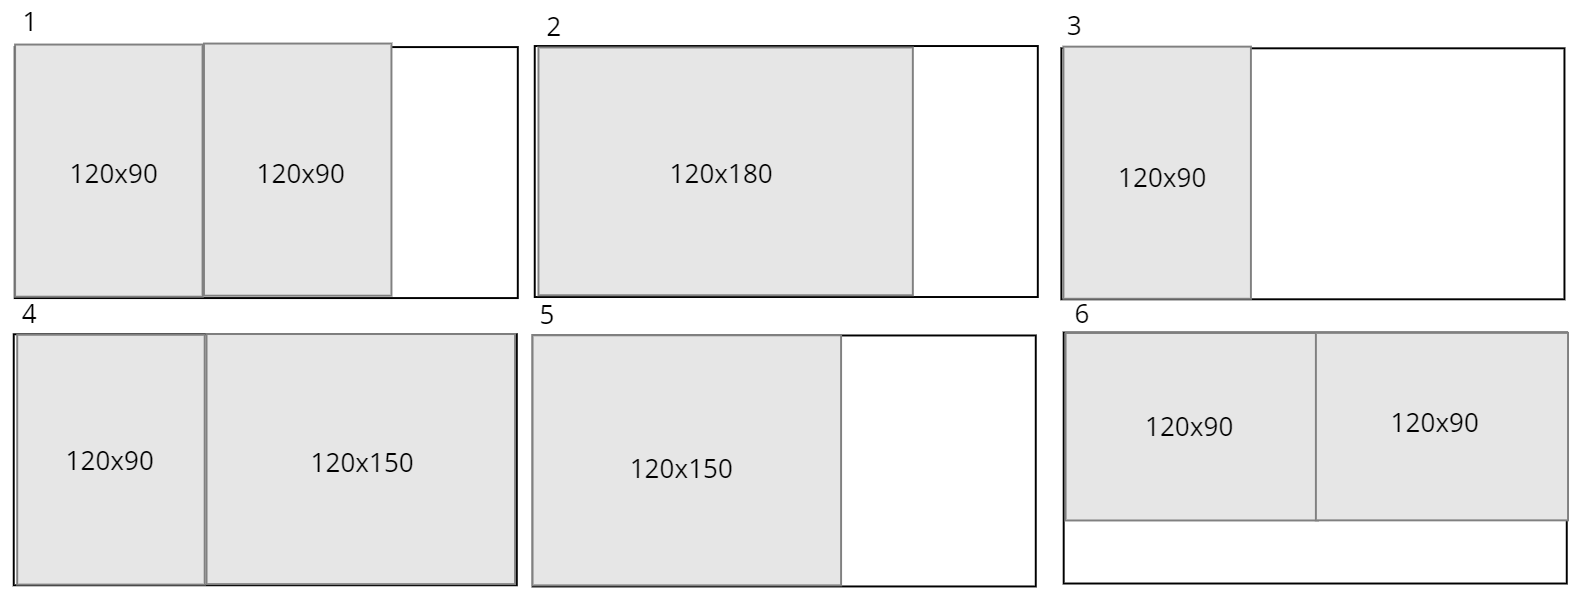
\includegraphics[scale=0.4]{img01}
	$$
	Причем заметим, что варианты 1 и 6 совпадают по прибыли, поэтому вариант 6 можно исключить. Вариант разреза 4 получается непосредственно из вариантов 3 и 5, поэтому их также можно исключить. Поскольку нам нужно 50 листов размера $120\times 150$, то, вырезая их по варианту 4, мы заведомо получаем и 50 листов размера $120\times 90$, поэтому вариант 1 также можно исключить. В итоге имеем 2 варианта разреза:
	$$
		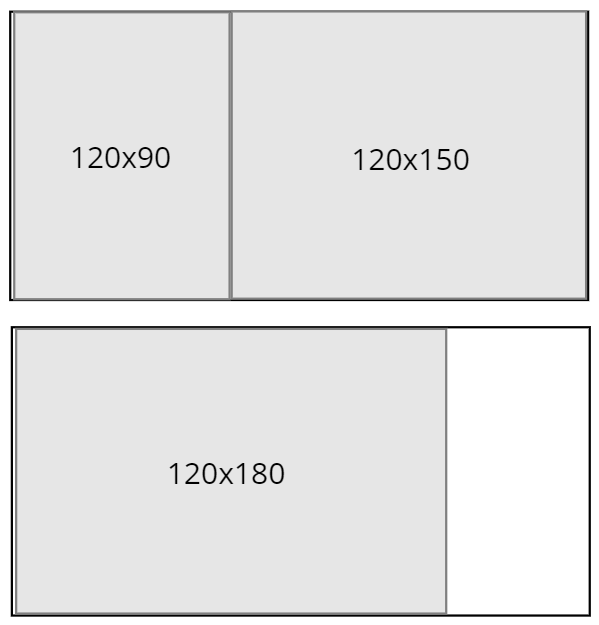
\includegraphics[scale=0.3]{img02}
	$$
	Введем обозначения
	\begin{itemize}
		\item $x_1$ --- количество листов оргалита $120\times 90$ см$^2$;
		\item $x_2$ --- количество листов оргалита $120\times 150$ см$^2$;
		\item $x_3$ --- количество листов оргалита $120\times 180$ см$^2$;
		\item $y_1$ --- количество больших листов для 1-го варианта разреза;
		\item $y_2$ --- количество больших листов для 2-го варианта разреза.
	\end{itemize}
	С учетом того, что, использовав один лист $y_i$ мы тратим 750 у.е (600 у.е. на покупку и 150 у.е. на разрез), 
	суммарная прибыль составляет $$z = 700x_1 + 900x_2 + 1000x_3 - 750y_1 - 750 y_2.$$
	Эта функция и будет являться целевой функцией, определяющей суммарную прибыль, которую мы должны максимизировать.\\\\
	Введем ограничения для переменных. Количество листов не может быть отрицательным, поэтому $$x_i \geq 0,\ i=1,2,3;\quad y_j \geq 0,\ j=1,2.$$
	Необходимо продать не менее определенного количества каждого из листов, причем учитывая также большие листы, получаем:
	$$x_1 + y_1 \geq 20,$$
	$$x_2 + y_1 \geq 50,$$
	$$x_3 + y_2 \geq 40.$$
	Таким образом, итоговая математическая модель имеет вид:
	$$z = 700x_1 + 900x_2 + 1000x_3 - 750y_1 - 750 y_2\to \max$$
	$$\begin{cases}
		x_1 + y_1 \geq 20,\\
		x_2 + y_1 \geq 50,\\
		x_3 + y_2 \geq 40;
	\end{cases}$$
	$$x_i \geq 0,\ y_j \geq 0,\quad i=1,2,3;\ j=1,2.$$
	Она описывает задачу линейного программирования.
	\subsection*{Реализация математической модели в форме файла .mod}
	Файл модели model.mod имеет следующую структуру:
	\listinginput[1]{1}{model.mod}
	\subsection*{Заполнение данными модели в форме файла .dat}
	Файл модели data.dat имеет следующую структуру:
	\listinginput[1]{1}{data.dat}
	\subsection*{Решение оптимизационной задачи средствами AMPL}
	Файл запуска clp.run имеет следующую структуру:
	\listinginput[1]{1}{clp.run}
	Ответ в окне консоли:
	\begin{verbatim}
		ampl: include clp.run
		CPLEX 22.1.1.0: integer unbounded ray.
		0 MIP simplex iterations
		0 branch-and-bound nodes
		No basis.
		z = 0
		
		x [*] :=
		1  0
		2  0
		3  0
		;
		
		y [*] :=
		1  0
		2  0
		;
	\end{verbatim}
	На выходе не получили решения, из-за того, что на задачу отсутствуют какие-либо ограничения сверху. Без каких-либо дополнительных условий будем считать, что, таким образом, мы можем постоянно увеличивать прибыль с продажи листов разрезанных выбранным образом.
\end{document}